\documentclass[fleqn, 12pt]{article}
\usepackage{fancyhdr}
\usepackage{amsmath}
\usepackage[utf8]{inputenc}
\usepackage[T2A]{fontenc}
\usepackage[english, russian]{babel}
\usepackage[left=10mm, top=20mm, right=10mm, bottom=20mm]{geometry}
\usepackage{lmodern}
\usepackage{erewhon}
\usepackage{multicol}
\usepackage{txfonts}
\usepackage{enumitem}
\usepackage{graphicx}
\graphicspath{ {./img/} }
\fancyhf{}
\fancyfoot[C]{\textbf{\thepage}}

\makeatletter
\renewcommand{\@seccntformat}[1]{}
\makeatother
\begin{document}
\newpage
\begin{titlepage}
    \fontsize{12pt}{14.4pt}
    \selectfont
    \begin{center}
        Федеральное государственное автономное
        образовательное учреждение высшего образования
        Национальный Исследовательский Университет ИТМО \\
        Факультет Программной Инженерии и Компьютерной Техники
    \end{center}

    \vspace{11em}

    \begin{center}
        \large{\textbf{ИДЗ №3} \linebreak
        Вариант: №17 \linebreak}
    \end{center}

    \vspace{18em}




    \hfill\parbox{10cm}{
        Выполнил:\hfill\hbox to 190pt{Назин Артем Аркадьевич\hfill}\\
        Группа:\hfill\hbox to 190pt{P3107\hfill}\\
        Поток:\hfill\hbox to 190pt{11.3\hfill}\\
        Преподаватель:\hfill\hbox to 190pt{Ершов Александр Романович\hfill}
    }


    \vspace{\fill}

    \begin{center}
        Город Санкт-Петербург \\2023
    \end{center}
    
\end{titlepage}
\setlength{\mathindent}{0.0pt}
\tableofcontents

\vfill
{\bf P.S.} Данное ИДЗ выполнено в \TeX \space и является моим вторым опытом работы в нём после Лабы №6 по информатике, 
так что прошу прощения за тонну орфографических ошибок и очень кривое оформление местами
\newpage
% \renewcommand{\labelenumi}{\latintext{enumi}}
\section{Задание 1}
 {\bf\large Условие} \\Построить эскиз графика данной функции, используя преобразования
графика соответствующей \\ элементарной функции. Указать область определения и область значений данной функции:
\begin{enumerate}
    \item $y =3\sin{\left(2+\frac{x}{2\pi}\right)}-5$
    \item $y =\sqrt{\left(\frac{|6-2x|+x}{10-|5x-15|}\right)^2}$
    \item $y =\log_4{\left(2+\sqrt{\frac{1}{x}}\right)}$
\end{enumerate}
{\bf\large Ход решения} 
\[
    1. \hspace{10pt} y =3\sin{\left(2+\frac{x}{2\pi}\right)}-5 = 3\sin{\left(\frac{(x+4\pi)}{2\pi}\right)}-5
\]
Построим базовую функцию: $y = \sin{x}$: \\
\begin{center}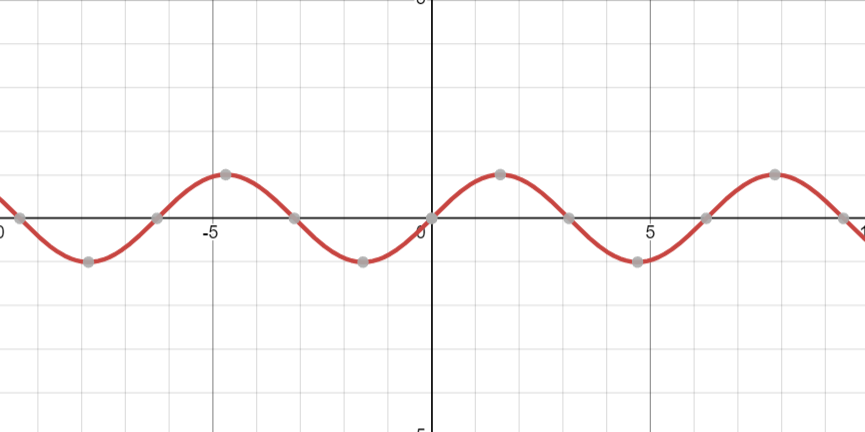
\includegraphics[width=0.7\linewidth]{1.png}\end{center}
Изменим циклическую частоту: $y = \sin{\left(\frac{x}{2\pi}\right)}$: \\
\begin{center}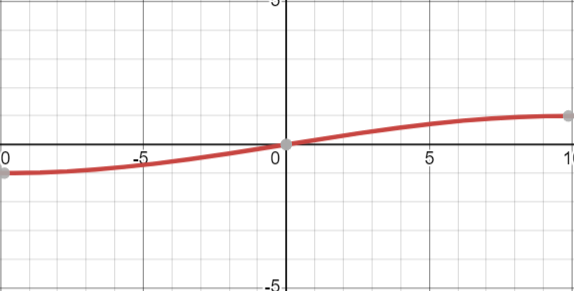
\includegraphics[width=0.7\linewidth]{2.png}\end{center}
Растянем график в 3 раза по OY: $y = 3\sin{\left(\frac{x}{2\pi}\right)}$:
\begin{center}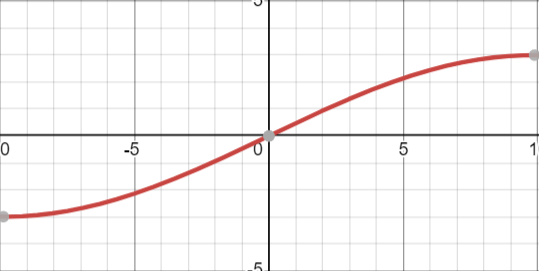
\includegraphics[width=0.7\linewidth]{3.png}\end{center}
Построим график относительно новых осей: 
$y' = y + 5$ и $x' = x + 4\pi$:
\begin{center}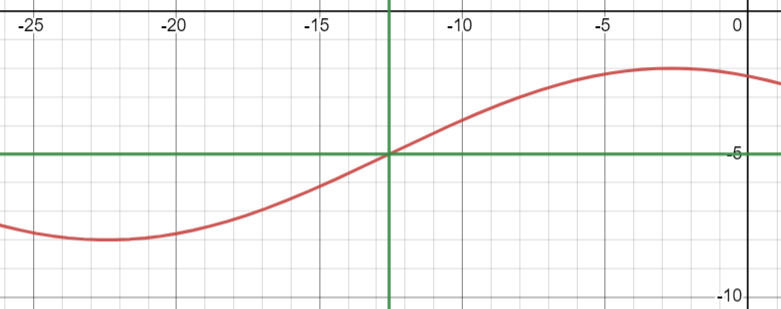
\includegraphics[width=0.7\linewidth]{4.png}\end{center}
В итоге, посредством элементарных преобразований мы получили график функции $y =3\sin{\left(2+\frac{x}{2\pi}\right)}-5$:
\begin{center}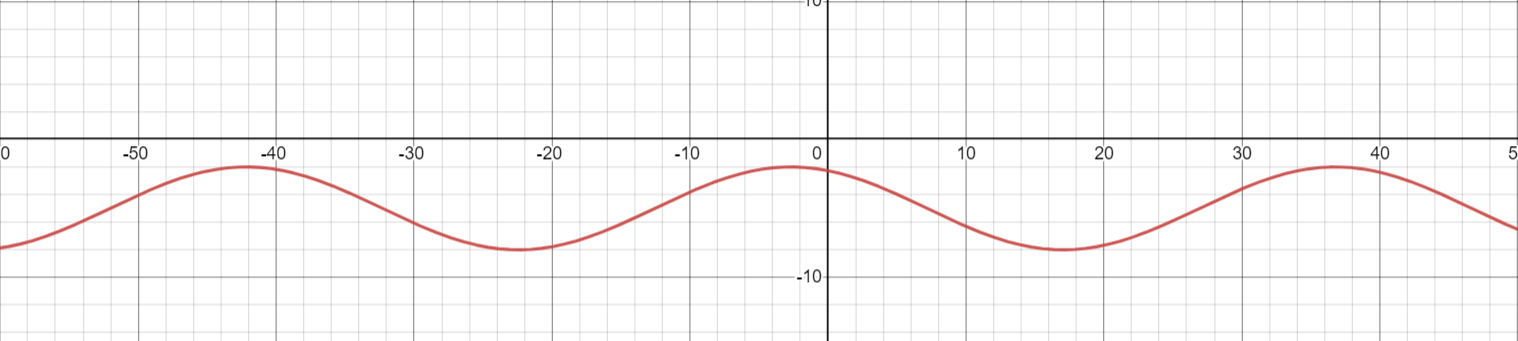
\includegraphics[width=0.7\linewidth]{5.png}\end{center}
\newpage
\[
    2. \hspace{10pt} y =\sqrt{\left(\frac{|6-2x|+x}{10-|5x-15|}\right)^2} = \left|\left(\frac{|6-2x|+x}{10-|5x-15|}\right)\right|
\]
\noindent Раскроем внутренние модули:
\begin{equation*}
    \begin{cases}
        \left|\frac{-x+6}{5x-5}\right|, x < 3 \hspace{20pt} (1)\\
        \left|\frac{3x-6}{-5x+25}\right|, x \geq 3  \hspace{12.5pt} (2)\\
    \end{cases}
\end{equation*}
\noindent Теперь построим $(1)$ и $(2)$ без модулей: \\
{\bf (1):} \\
$\frac{3x-6}{-5x+25}=-\frac{1}{5}+\frac{1}{x-1}$ \\
\noindent Для этого сначала построим базовый график $\frac{1}{x}$: 
\begin{center}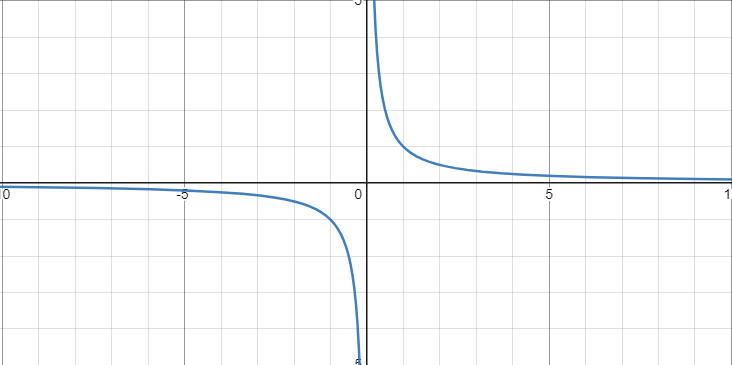
\includegraphics[width=0.7\linewidth]{7.png}\end{center}
После сместим на $+1$ по $x$ и $-\frac{1}{5}$ по $y$:
\begin{center}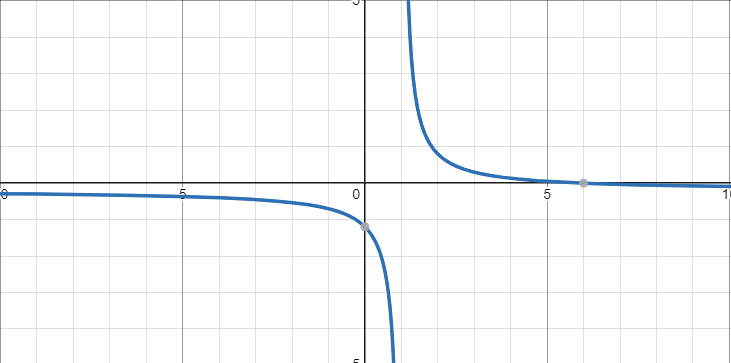
\includegraphics[width=0.7\linewidth]{8.png}\end{center}
\newpage
\noindent Уберем лишнее:
\begin{center}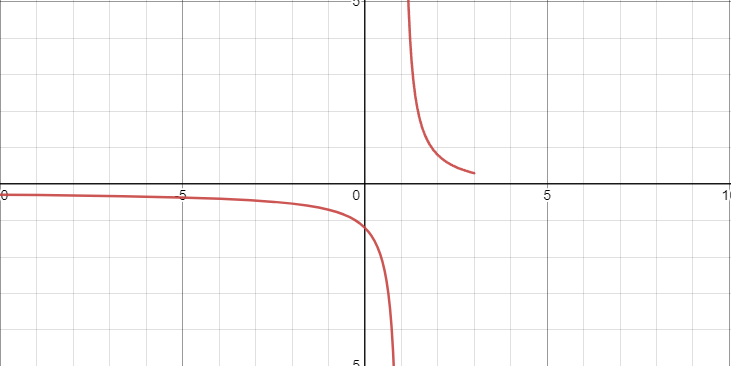
\includegraphics[width=0.7\linewidth]{9.png}\end{center}
Аналогично для {\bf (2):}  \\
$\frac{3x-6}{-5x+25}=-\frac{3}{5}+\frac{9}{-5(x-5)}$ \\
\begin{center}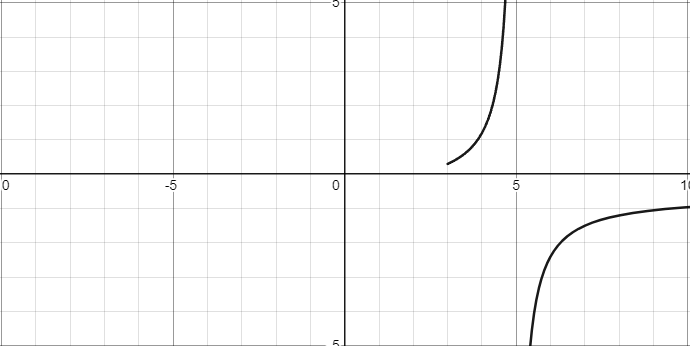
\includegraphics[width=0.7\linewidth]{10.png}\end{center}
\newpage
\noindent Совместим и отразим отрицательную часть относительно оси OX, то есть получим итоговый график:
\begin{center}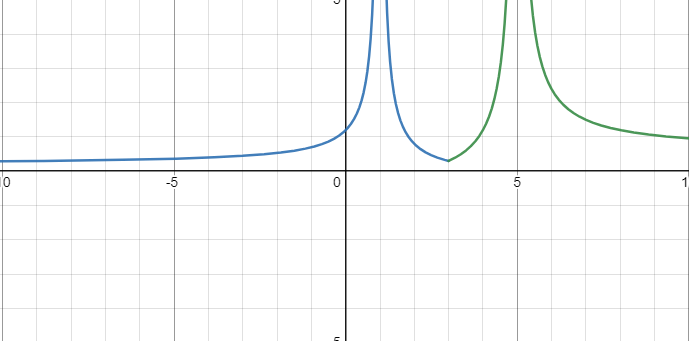
\includegraphics[width=0.7\linewidth]{11.png}\end{center}
\[3. \hspace{10pt} y =\log_4{\left(2+\sqrt{\frac{1}{x}}\right)}\]
График этой функции построим, изучив предварительно ее свойства. \\
Функция определена для $x>0$ и монотонно убывает от $+\infty$ до $0.5$ \\
Построим поочередно графики. Сначала $\frac{1}{x}$ (красная линия), потом  $2+\sqrt{\frac{1}{x}}$ (синия линия), следом     $\log_4{\left(2+\sqrt{\frac{1}{x}}\right)}$ (черная линия):
\begin{center}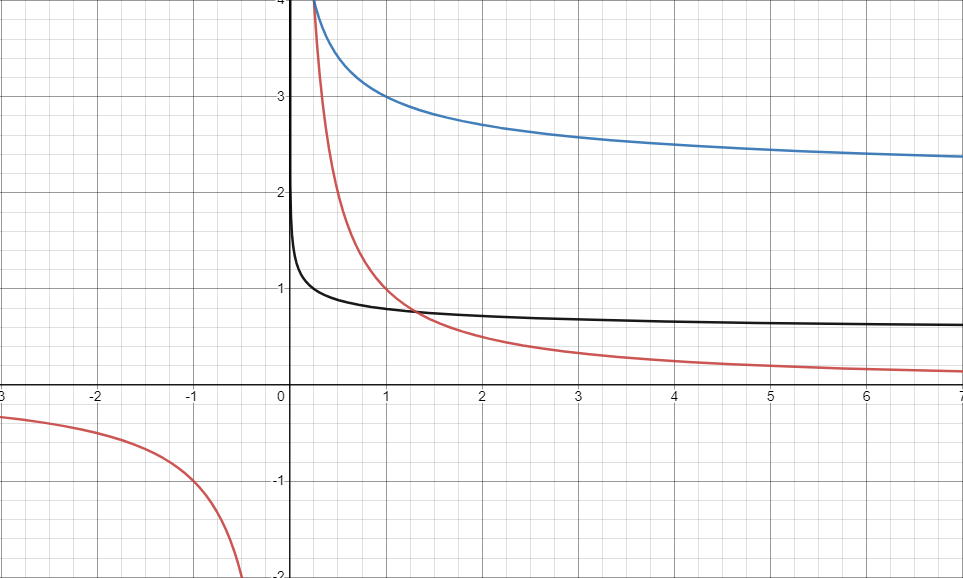
\includegraphics[width=0.7\linewidth]{12.png}\end{center}

\newpage
\section{Задание 2} 
{\bf\large Условие} \\
Доказать по определению предела функции в точке (по Коши):
\[
    \lim_{x\rightarrow11}{\frac{2x^2-21x-11}{x-11}}=23
\]
{\bf\large Ход решения} 
Преобразуем выражение $\left|\frac{2x^2-21x-11}{x-11}-23\right|$:
\[
    \left|\frac{2x^2-21x-11}{x-11}-23\right|=\left|\frac{2x^2-21x-11-23x+253}{x-11}\right|=\left|\frac{2x^2-44x+242}{x-11}\right|=\left|\frac{2(x-11)^2}{x-11}\right|
\]
Так как при стремлении к $11$, $x$ в саму точку $11$ не попадает, то:
\[
    \left|\frac{2(x-11)^2}{x-11}\right| = 2\left|x-11\right|
\]
Возьмем $\varepsilon$ > 0 и найдем решения неравенства:
\[
    \left|\frac{2x^2-21x-11}{x-11}-23\right| = 2\left|x-11\right| < \varepsilon
\]
\[    
    \left|x-11\right| < \frac{\varepsilon}{2}
\]
Получается, что из неравенства $\left|x-11\right| < \frac{\varepsilon}{2}$ следует $\left|\frac{2x^2-21x-11}{x-11}-23\right| < \varepsilon$, то есть выполнено определение предела по Коши для $\delta =  \frac{\varepsilon}{2}$. ч.т.д.

\newpage
\section{Задание 3} 
{\bf\large Условие} \\
Доказать, что данный предел не существует:
\[
    \lim_{x\rightarrow\infty}{\ctg{(1+x^2)}}
\]
{\bf\large Ход решения} \\
Рассмотрим некоторые последвательности $x_n$ удовлетворяющие первой части определения по Гейне, то есть такие что:
\begin{equation*}
    \begin{cases}
        x_n \in D(f) \text{ (Область определения)} \\
        x_n \rightarrow +\infty
    \end{cases}
\end{equation*}
Например: $y_n = \sqrt{\frac{\pi}{4}+\pi n -1}$ и $a_n = \sqrt{\frac{3\pi}{4}+\pi n -1}$. К тому же $n\geq1\Rightarrow y_n,a_n\geq 0$. \\
Получается $\ctg{(1+y_n^2)}= \ctg{\left(1+\left(\sqrt{\frac{\pi}{4}+\pi n -1}\right)^2\right)}=\ctg{\left(1+\frac{\pi}{4}+\pi n -1\right)}=\ctg{\left(\frac{\pi}{4}+\pi n\right)}=\ctg{\frac{\pi}{4}}=const=1$\\
А $\ctg{(1+a_n^2)} = \ctg{\left(1+\left(\sqrt{\frac{3\pi}{4}+\pi n -1}\right)^2\right)}=\ctg{\left(1+\frac{3\pi}{4}+\pi n -1\right)}=\ctg{\left(\frac{3\pi}{4}+\pi n\right)}=\ctg{\frac{3\pi}{4}}=const=-1$\\
То есть мы взяли две последовательности из определения по Гейне и получили, что они стремятся к разным числам, что напрямую этому определению противоречит, следовательно предела - нет. ч.т.д. \\
Аналогично для $x \rightarrow -\infty$.

\newpage
\section{Задание 4}
 {\bf\large Условие} \\Вычислить пределы:
\begin{multicols}{2}
    \begin{enumerate}
        \item
              \[
                  \lim_{x\rightarrow -1}{\frac
                      {x^3-3x-2}
                      {(x^2-x-2)^2}}
              \]
        \item
              \[
                  \lim_{x\rightarrow  3}{\frac
                      {\sqrt[3]{9x}-3}
                      {\sqrt{3+x}-\sqrt{2x}}}
              \]
        \item
              \[
                  \lim_{x\rightarrow 1}{\frac
                  {1+\cos{\pi x}}
                  {\tg^2{\pi x}}}
              \]
        \item
              \[
                  \lim_{x\rightarrow a}{\frac
                  {\ln{( \cos{\frac{\pi x}{a}}+2)}}
                  {a^{\frac{a^2}{x^2}-\frac{a}{x}}-a^{\frac{a}{x}-1}}}
              \]
        \item
              \[
                  \lim_{x\rightarrow  0}{
                  (2-5^{\arcsin{x^3}})^\frac{(\cosec^2{x})}{x}
                  }
              \]
        \item
              \[
                  \lim_{x\rightarrow  \frac{\pi}{2} \pm 0}{
                      (0.5+\cos{3x})^{\sec{x}}
                  }
              \]
        \item
              \[
                  \lim_{x\rightarrow  \frac{\pi}{2}}{
                      \frac{2+\cos{x}\sin{\frac{2}{2x-\pi}}}{3+2x\sin{x}}
                  }
              \]
        \item
              \[
                  \lim_{x\rightarrow  2}{
                      \frac{\arctg{(x^2-3)}+\arctg{(x^2-5)}}{\ln{(x-1)}}
                  }
              \]
    \end{enumerate}
\end{multicols}
\newpage
{\bf\large Ход решения}
\begin{enumerate}
    \item
          \begin{gather*}
              \lim_{x\rightarrow -1}{\frac
                  {x^3-3x-2}
                  {(x^2-x-2)^2}} \\
              \text{Вид неопределенности: }{\left[\frac{0}{0}\right]} \\
              \lim_{x\rightarrow -1}{\frac
                  {x^3-3x-2}
                  {(x^2-x-2)^2}} =
              \lim_{x\rightarrow -1}{\frac
                  {(x^2-x-2)(x+1)}
                  {(x^2-x-2)^2}} =
              \lim_{x\rightarrow -1}{\frac
                  {x+1}
                  {x^2-x-2}} =
              \lim_{t\rightarrow 0}{\frac
                  {t-1+1}
                  {(t-1)^2-(t-1)-2}} = \\ =
              \lim_{t\rightarrow 0}{\frac
                  {t}
                  {t^2-2t+1-t+1-2}} =
              \lim_{t\rightarrow 0}{\frac
                  {t}
                  {t^2-3t}} =
              \lim_{t\rightarrow 0}{\frac
                  {\frac{t}{t}}
                  {\frac{t^2}{t}-\frac{3t}{t}}} =
              \lim_{t\rightarrow 0}{\frac
                  {1}
                  {t-3}} =
              -\frac{1}{3}
          \end{gather*}
          {\bf Ответ:} $-\frac{1}{3}$
    \item
          \begin{gather*}
              \lim_{x\rightarrow 3}{\frac
                  {\sqrt[3]{9x}-3}
                  {\sqrt{3+x}-\sqrt{2x}}} \\
              \text{Вид неопределенности: }{\left[\frac{0}{0}\right]} \\
              \lim_{x\rightarrow 3}{\frac
                  {\sqrt[3]{9x}-3}
                  {\sqrt{3+x}-\sqrt{2x}}} =
              \lim_{t\rightarrow 0}{\frac
                  {\sqrt[3]{9t+27}-3}
                  {\sqrt{t+6}-\sqrt{2t+6}}} =
              \lim_{t\rightarrow 0}{\frac
                  {3\sqrt[3]{\frac{t}{3}+1}-3}
                  {\sqrt{6}\sqrt{\frac{t}{6}+1}-\sqrt{6}\sqrt{\frac{t}{3}+1}}} = \\
              = \lim_{t\rightarrow 0}{\frac
              {3(1+\frac{t}{9}+o(t))-3}
              {\sqrt{6}(1+\frac{t}{12}+o(t))-\sqrt{6}(1+\frac{t}{6}+o(t))}} =
              \lim_{t\rightarrow 0}{\frac
                  {\frac{t}{3}+o(t)}
                  {\frac{\sqrt{6}t}{12}-\frac{\sqrt{6}t}{6}+o(t)}} =
              \lim_{t\rightarrow 0}{\frac
                  {\frac{t}{3}+o(t)}
                  {-\frac{\sqrt{6}t}{12}+o(t)}} = \\
              = \lim_{t\rightarrow 0}{\frac
                  {\frac{1}{3}+o(1)}
                  {-\frac{\sqrt{6}}{12}+o(1)}} =
              \frac{\frac{1}{3}}{-\frac{\sqrt{6}}{12}} =
              -\frac{2\sqrt{6}}{3}
          \end{gather*}
          {\bf Ответ:} $-\frac{2\sqrt{6}}{3}$
    \item
          \begin{gather*}
              \lim_{x\rightarrow  1}{\frac
              {1+\cos{\pi x}}
              {\tg^2{\pi x}}} \\
              \text{Вид неопределенности: }{\left[\frac{0}{0}\right]} \\
              \lim_{x\rightarrow  1}{\frac
              {1+\cos{\pi x}}
              {\tg^2{\pi x}}} =
              \lim_{t\rightarrow  0}{\frac
              {1+\cos{\pi t + \pi}}
              {\tg^2{\pi t + \pi}}} =
              \lim_{t\rightarrow  0}{\frac
              {1-\cos{\pi t}}
              {\tg^2{\pi t}}} =
              \lim_{t\rightarrow  0}{\frac
                  {1-(1-\frac{\pi^2 t^2}{2}+o(t^2))}
                  {(\pi t + o(t))^2}} = \\
              = \lim_{t\rightarrow  0}{\frac
                  {\frac{\pi^2 t^2}{2}+o(t^2)}
                  {\pi^2 t^2 + o(t) \pi t+ o(t^2)}} =
              \lim_{t\rightarrow  0}{\frac
                  {\frac{\pi^2 t^2}{2}+o(t^2)}
                  {\pi^2 t^2 + o(t^2)}} =
              \lim_{t\rightarrow  0}{\frac
                  {\frac{\pi^2}{2}+o(1)}
                  {\pi^2 + o(1)}} =
              \frac{1}{2}
          \end{gather*}
          {\bf Ответ:} $\frac{1}{2}$
          \newpage
    \item
          \begin{gather*}
              \lim_{x\rightarrow  a}{\frac
              {\ln{( \cos{\frac{\pi x}{a}}+2)}}
              {a^{\frac{a^2}{x^2}-\frac{a}{x}}-a^{\frac{a}{x}-1}}}\\
              \text{Вид неопределенности: }{\left[\frac{0}{0}\right]} \\
              \lim_{x\rightarrow  a}{\frac
              {\ln{( \cos{\frac{\pi x}{a}}+2)}}
              {a^{\frac{a^2}{x^2}-\frac{a}{x}}-a^{\frac{a}{x}-1}}} =
              \lim_{x\rightarrow  a}{\frac
                  {\ln{( \cos{\frac{\pi x}{a}}+2)}}
                  {a^{\frac{a}{x}-1}\left(a^{\frac{a^2}{x^2}-\frac{2a}{x}+1}-1\right)}} =
              \lim_{t\rightarrow  0}{\frac
                  {\ln{( \cos{\frac{\pi (t+a)}{a}}+2)}}
                  {a^{\frac{a}{t+a}-1}\left(a^{\frac{a^2}{(t+a)^2}-\frac{2a}{t+a}+1}-1\right)}} = \\
              = \lim_{t\rightarrow  0}{\frac
                  {\ln{( \cos{(\frac{\pi t}{a}+\pi)}+2)}}
                  {a^{\frac{a-t-a}{t+a}}\left(a^{\frac{a^2}{(t+a)^2}-\frac{2at+2a^2}{(t+a)^2}+\frac{(t+a)^2}{(t+a)^2}}-1\right)}} =
              \lim_{t\rightarrow  0}{\frac
                  {\ln{( -\cos{\frac{\pi t}{a}}+2)}}
                  {a^{\frac{-t}{t+a}}\left(a^{\frac{a^2-2at-2a^2+t^2+2at+a^2}{(t+a)^2}}-1\right)}} = \\
              = \lim_{t\rightarrow  0}{\frac
                  {\ln{( -\cos{\frac{\pi t}{a}}+2)}}
                  {a^{\frac{-t}{t+a}}\left(a^{\frac{t^2}{(t+a)^2}}-1\right)}} =
              \lim_{t\rightarrow  0}{\frac
                  {\ln{( -(1-\frac{\pi^2 t^2}{2a^2}+o(t^2))+2)}}
                  {\left(1-\frac{t}{t+a}\ln(a)+o(t)\right)\left((1+\frac{t^2}{(t+a)^2}\ln(a)+o(t^2))-1\right)}} = \\
              = \lim_{t\rightarrow  0}{\frac
                  {\ln{(1+\frac{\pi^2 t^2}{2a^2}+o(t^2))}}
                  {\left(1-\frac{t}{t+a}\ln(a)+o(t)\right)\left(\frac{t^2}{(t+a)^2}\ln(a)+o(t^2)\right)}} =\\
              = \lim_{t\rightarrow  0}{\frac
                  {\frac{\pi^2 t^2}{2a^2}+o(t^2)+o(\frac{\pi^2 t^2}{2a^2}+o(t^2))}
                  {\frac{t^2}{(t+a)^2}\ln(a)+o(t^2)-\frac{t^3}{(t+a)^3}\ln^2(a)-\frac{t}{t+a}o(t^2)+\frac{t^2}{(t+a)^2}\ln(a)o(t)+o(t)o(t^2)}} \\
              \text{Заметим, что: } o\left(\frac{t^k}{(a+t)^n}\right)=o(t^k) \text{, где k,n}  \in \mathbb{N} \text{ (ограниченная умножить на  } t^k \text{ )}\\
              \text{Откуда: }
              \lim_{t\rightarrow  0}{\frac
                  {\frac{\pi^2 t^2}{2a^2}+o(t^2)+o(\frac{\pi^2 t^2}{2a^2}+o(t^2))}
                  {\frac{t^2}{(t+a)^2}\ln(a)+o(t^2)-\frac{t^3}{(t+a)^3}\ln^2(a)-o(t^3)+o(t^3)}} =
              \lim_{t\rightarrow  0}{\frac
                  {\frac{\pi^2 t^2}{2a^2}+o(t^2)}
                  {\frac{t^2}{(t+a)^2}\ln(a)+o(t^2)-\frac{t^3}{(t+a)^3}\ln^2(a)}} = \\
              = \lim_{t\rightarrow  0}{\frac
                  {\frac{\pi^2}{2a^2}+o(1)}
                  {\frac{1}{(t+a)^2}\ln(a)+o(1)-\frac{t}{(t+a)^3}\ln^2(a)}} =
              \frac
              {\frac{\pi^2}{2a^2}}
              {\frac{1}{a^2}\ln(a)-0} =
              \frac{\pi^2}{2\ln(a)}
          \end{gather*}
          {\bf Ответ:} $\frac{\pi^2}{2\ln(a)}$
    \item
          \begin{gather*}
              \lim_{x\rightarrow  0}{
              (2-5^{\arcsin{x^3}})^\frac{(\cosec^2{x})}{x}} \\
              \text{Вид неопределенности: }{\left[1^{\infty}\right]} \\
              \lim_{x\rightarrow  0}{
              (2-5^{(x^3+o(x^3))})^\frac{1}{x\sin^2{x}}} =
              \lim_{x\rightarrow  0}{
              (2-5^{(x^3+o(x^3))})^\frac{1}{x(x+o(x))^2}} =
              \lim_{x\rightarrow  0}{
                  (2-(1+(x^3+o(x^3))\ln{5}+o(x^3+o(x^3))))^\frac{1}{x^3+o(x^3)}} = \\
              = \lim_{x\rightarrow  0}{
                  (1-x^3\ln{5}+o(x^3))^{\left(\frac{1}{-x^3\ln{5}+o(x^3)}\frac{-x^3\ln{5}+o(x^3)}{x^3+o(x^3)}\right)}} =
              \lim_{x\rightarrow  0}{
                  e^{\left(\frac{-x^3\ln{5}+o(x^3)}{x^3+o(x^3)}\right)}} =
              \lim_{x\rightarrow  0}{
                  e^{\left(\frac{-\ln{5}+o(1)}{1+o(1)}\right)}} =
              e^{-\ln{5}} = \frac{1}{5}
          \end{gather*}
          {\bf Ответ:} $\frac{1}{5}$
    \item
          \begin{gather*}
              \lim_{x\rightarrow  \frac{\pi}{2} \pm 0}{
                  (0.5+\cos{3x})^{\sec{x}}} \\
              \\
              \lim_{x\rightarrow  \frac{\pi}{2} \pm 0}{
                  (0.5+\cos{3x})^{\sec{x}}} =
              \lim_{t\rightarrow  0 \pm }{
              \left(0.5+\cos{\left(3t+\frac{3\pi}{2}\right)}\right)^{\frac{1}{\cos{\left(\frac{\pi}{2}+t\right)}}}} =
              \lim_{t\rightarrow  0 \pm }{
                  (0.5+\sin{3t})^{\frac{1}{-\sin{t}}}} \\
              \text{Рассмотрим отдельно при } t \rightarrow 0+ \text{ и } t \rightarrow 0- \\
              \lim_{t\rightarrow  0- }{
                  (0.5+\sin{3t})^{\frac{1}{-\sin{t}}}} =
              \lim_{t\rightarrow  0- }{
                  (0.5+3t+o(t))^{\frac{1}{-(t+o(t))}}} =
              \lim_{t\rightarrow  0- }{
                  (0.5+3t+o(t))^{\infty}} =
              \lim_{t\rightarrow  0- }{
                  (0.5)^{\infty}} = 0 \\
              \lim_{t\rightarrow  0+ }{
                  (0.5+\sin{3t})^{\frac{1}{-\sin{t}}}} =
              \lim_{t\rightarrow  0+ }{
                  (0.5+3t+o(t))^{\frac{1}{-(t+o(t))}}} =
              \lim_{t\rightarrow  0+ }
              (0.5+3t+o(t))^{-\infty} =
              \lim_{t\rightarrow  0+ }
              (0.5)^{-\infty} = +\infty
          \end{gather*}
          {\bf Ответ для $x\rightarrow \frac{\pi}{2}-0$: $0$, \\ для $x\rightarrow \frac{\pi}{2}+0$: $+\infty$}
    \item
          \begin{gather*}
              \lim_{x\rightarrow  \frac{\pi}{2}}{
                  \frac{2+\cos{x}\sin{\frac{2}{2x-\pi}}}{3+2x\sin{x}}} \\
              \\
              \lim_{x\rightarrow  \frac{\pi}{2}}{
                  \frac{2+\cos{x}\sin{\frac{2}{2x-\pi}}}{3+2x\sin{x}}} =
              \lim_{t\rightarrow  0}{
                  \frac{2+\cos{(t+\frac{\pi}{2})}\sin{\frac{2}{2t+\pi-\pi}}}{3+2(t+\frac{\pi}{2})\sin{\left(t+\frac{\pi}{2}\right)}}} = \frac{2-\sin{t}\sin{\frac{2}{2t}}}{3+2(t+\frac{\pi}{2})\cos{t}} \\
              \text{Функция: } \sin{\frac{1}{t}} \text{ - ограниченная, а } \sin{t} \text{ - бесконечно малая} \\ \text{Следовательно их произведение - бесконечно малая} \\
              \text{Откуда. подставив $t = 0$, получим: } \\
              \frac{2-0}{3+2(0+\frac{\pi}{2})\cos{(0)}} = \frac{2}{3+\pi}
          \end{gather*}
          {\bf Ответ: $\frac{2}{3+\pi}$}
    \item
          \begin{gather*}
              \lim_{x\rightarrow  2}{
                  \frac{\arctg{(x^2-3)}+\arctg{(x^2-5)}}{\ln{(x-1)}}
              } \\
              \lim_{x\rightarrow  2}{
                  \frac{\arctg{(x^2-3)}+\arctg{(x^2-5)}}{\ln{(x-1)}}
              } = 
              \lim_{t\rightarrow  0}{
                  \frac{\arctg{(t^2+4t+4-3)}+\arctg{(t^2+4t+4-5)}}{\ln{(t+1)}}
              } =\\=
              \lim_{t\rightarrow  0}{
                  \frac{\arctg{(t^2+4t+1)}+\arctg{(t^2+4t-1)}}{\ln{(t+1)}}
              } =
              \lim_{t\rightarrow  0}{
                  \frac{f_1(t)+f_2(t)}{h(t)}
              }
              \\
              \text{Раскроем $arctg$ и $ln$ до первого порядка по формуле Тейлора, для этого посчитаем производные: } \\
              f_1'(t)=\left(\arctg{(t^2+4t+1)}\right)' = \frac{2t+4}{1+(t^2+4t+1)^2} \\
              f_2'(t)=\left(\arctg{(t^2+4t-1)}\right)' = \frac{2t+4}{1+(t^2+4t-1)^2} \\
              h'(t)=\left(\ln{(t+1)}\right)' = \frac{1}{t+1} \\
              \text{Подставим $t_0$:} \\
              f_1(0) = \arctg{(0^2+4*0+1)} = \arctg{(1)} = \frac{\pi}{4} \\
              f_2(0) = \arctg{(0^2+4*0-1)} = \arctg{(-1)} = -\frac{\pi}{4} \\
              h(0) = \ln{(0+1)} = \ln{(1)} = 0 \\
              f_1'(0) = \frac{2*0+4}{1+(0^2+0*t+1)^2} = \frac{4}{1+1^2} = 2 \\
              f_2'(0) = \frac{2*0+4}{1+(0^2+0*t-1)^2} = \frac{4}{1+(-1)^2} = 2 \\
              h'(0) = \frac{1}{0+1} = 1 \\
              \text{Откуда:} \\
              \lim_{t\rightarrow  0}{
                  \frac{f_1(t)+f_2(t)}{h(t)}
              } = 
              \lim_{t\rightarrow  0}{
                  \frac{\left(\frac{\pi}{4}+2t+o(t)\right)+\left(-\frac{\pi}{4}+2t+o(t)\right)}
                  {0+t+o(t)}
              } = 
              \lim_{t\rightarrow  0}{
                \frac{4t+o(t)}{t+o(t)}
              } = 
              \lim_{t\rightarrow  0}{
                \frac{4+o(1)}{1+o(1)}
              } = 4
          \end{gather*}
          {\bf Ответ: $4$}
\end{enumerate}

\newpage
\section{Задание 5} 
{\bf\large Условие} \\
Провести полное исследование функций и построить их графики.
\begin{enumerate}
    \item 
    \begin{equation*}
        \begin{cases}
            x = \frac{3t^2 +1}{3t} \\
            y = t + \frac{t^2}{3}
        \end{cases}
    \end{equation*}
    \item 
    \[
        y = \arccos{\frac{2x}{1+x^2}} - \frac{2x}{5}
    \]
    \item 
    \[
        y = (1-x)e^{3x+1}
    \]
\end{enumerate}
{\bf\large Ход решения} \\
\begin{enumerate}
    \item 
    \begin{equation*}
        \begin{cases}
            x = \frac{3t^2 +1}{3t} \\
            y = t + \frac{t^2}{3}
        \end{cases}
    \end{equation*}
    Найдем область определения функции $D(f)$: \\
    $y(t)$ - существует всегда, рассмотрим чему не может равняться $x(t)$:\\
    $x(t) = \frac{3t^2 +1}{3t} = t + \frac{1}{3t}$ - не достигает каких-то значений около нуля, найдем их через локальный минимум/максимум: \\
    $x'(t) = 1 - \frac{1}{3t^2}$ - не существует в нуле как и сама функция $x(t)$,
    $x'(t) = 0 \Rightarrow 1 - \frac{1}{3t^2} = 0 \Rightarrow t = \pm \sqrt{\frac{1}{3}}$ \\
    Подставив различные значения, получим, что: $\frac{1}{\sqrt{3}}$ - лок. минимум, $-\frac{1}{\sqrt{3}}$ - лок. максимум \\
    $x(\frac{1}{\sqrt{3}}) = \frac{2}{\sqrt{3}}$, $x(-\frac{1}{\sqrt{3}}) = -\frac{2}{\sqrt{3}}$ \\
    То есть $D(f) = (-\infty,-\frac{2}{\sqrt(3)}] \cup [\frac{2}{\sqrt(3)},+\infty)$ \\
    Найдем сначала асимптоты кривой. Будем искать наклонные асимптоты в виде $y = kx + b$. Переменная $x$ стремится к бесконечности, когда $t\rightarrow 0$ или $t\rightarrow \pm \infty$. 
    При $t \rightarrow \pm \infty$ переменная $y$ тоже будет стремится к бесконечности, при этом: \\
    \[
        \lim_{t\rightarrow \infty }{\frac{y(t)}{x(t)}} = \lim_{t\rightarrow \infty }{\frac{3t(3t+t^2)}{3(3t^2+1)}}
    \] 
    \item 
    \[
        y = \arccos{\frac{2x}{1+x^2}} - \frac{2x}{5}
    \]
    \item 
    \[
        y = (1-x)e^{3x+1}
    \]
\end{enumerate}

\newpage
\section{Задание 6}
{\bf\large Условие}\\
Из полосы жести шириной $a$ требуется сделать открытый сверху
желоб, поперечное сечение которого должно иметь форму равнобочной
трапеции. Дно желоба имеет ширину $b$. Какова должна быть ширина
желоба наверху, чтобы он вмещал наибольшее количество воды? \\
\\
{\bf\large Ход решения}
\begin{center}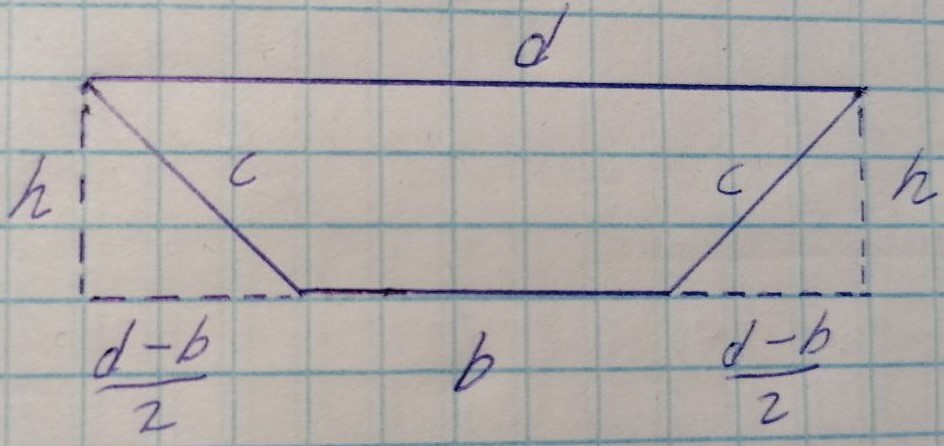
\includegraphics[width=0.7\linewidth]{6.jpg}\end{center}
Где $c = \frac{a-b}{2}$. \\
По теореме Пифагора: $c^2 = h^2 + \left(\frac{d-b}{2}\right)^2 \Rightarrow \left(\frac{a-b}{2}\right)^2 = h^2 + \left(\frac{d-b}{2}\right)^2
\Rightarrow h = \sqrt{\frac{(a-b)^2-(d-b)^2}{4}} = \sqrt{\frac{a^2-2ab-d^2+2db}{4}}$ \\
Площадь трапеции: $S = \frac{b+d}{2}\cdot h = \frac{b+d}{2} \cdot \sqrt{\frac{a^2-2ab-d^2+2db}{4}}$ \\
Желоб будет вмещать наибольший объем воды при фиксированной длине, если площадь сечения (трапеции) будет максимальной, найдем это максимальное значение с помощью производной: \\
$S' = \frac{1}{2} \sqrt{\frac{a^2-2ab-d^2+2db}{4}} + \frac{b+d}{2} \cdot \frac{-2d+2b}{4} \cdot \frac{1}{2} \cdot \frac{1}{\sqrt{\frac{a^2-2ab-d^2+2db}{4}}}$ \\
Из построения видно, что если $d \rightarrow a-$ то объем воды $=0$. 
К тому же, если $d\rightarrow0+$ то трапеция будет стремится к треугольнику, у которого площадь явно меньше. 
Значит, максимальное значение $S(d)$ будет в какой-нибудь точке локального максимума, найдем их: \\
\linebreak
\noindent Случай 1 ($S'(d)$ - не существует): \\
То есть $\frac{a^2-2ab-d^2+2db}{4}\leq0 \Rightarrow -d^2 + 2db +a^2-2ab\leq 0 \Rightarrow -(d-a)(d+a-2b)\leq 0 \Rightarrow (d-a)(d+a-2b)\geq 0$ \\
Откуда, по методу интерваллов получим, что либо $d\geq a$, либо $d\leq 2b-a$. \\
Первое невозможно так как если $d\geq a$, то трапецию не построишь (даже если боковые стороны "выпрямим" \space к основанию, то их все равно не хватит, чтобы достать до концов отрезка длиной d). \\
А $d\leq 2b-a\Leftrightarrow b+2c \leq 2b -d \Leftrightarrow c \leq \frac{b -d}{2} \Rightarrow c^2 \leq \left(\frac{b -d}{2}\right)^2 \Leftrightarrow \left(\frac{d-b}{2}\right)^2+h^2 \leq \left(\frac{b -d}{2}\right)^2 \Leftrightarrow h^2 \leq 0$ - чего не может быть. 
\newpage
\noindent Случай 2 ($S'(d) = 0$ ): \\
\begin{gather*}
    \frac{1}{2} \sqrt{\frac{a^2-2ab-d^2+2db}{4}} + \frac{b+d}{2} \cdot \frac{-2d+2b}{4} \cdot \frac{1}{2} \cdot \frac{1}{\sqrt{\frac{a^2-2ab-d^2+2db}{4}}} = 0 \\
    \sqrt{\frac{a^2-2ab-d^2+2db}{4}} = \frac{b+d}{2} \cdot \frac{d-b}{2} \cdot \frac{1}{\sqrt{\frac{a^2-2ab-d^2+2db}{4}}} \\
    \left(\sqrt{\frac{a^2-2ab-d^2+2db}{4}}\right)^2 = \frac{(d^2-b^2)}{4}\\
    a^2-2ab-d^2+2db= (d^2-b^2)\\
    2d^2-2bd-(a-b)^2=0
\end{gather*}
Решим квадратное уравнение относительно $d$:
\begin{gather*}
    D = 4b^2+8(a-b)^2 \text{ - сумма квадратов всегда неотрицательна}\\
    d_1 = \frac{2b+\sqrt{4b^2+8(a-b)^2}}{4}\\
    d_2 = \frac{2b-\sqrt{4b^2+8(a-b)^2}}{4} \text{ - явно меньше нуля, чего не может быть}
\end{gather*}
Итого $d = \frac{2b+\sqrt{4b^2+8(a-b)^2}}{4}$, докажем, что это максимум взяв, например $S'\left(\frac{b}{2}\right)$ и $S'\left(\frac{a-b}{\sqrt{2}}+b\right)$ \\
Расчеты, пожалуй опустим ;)\\
{\bf Ответ:} $d = \frac{2b+\sqrt{4b^2+8(a-b)^2}}{4}$


\newpage
\section{Задание 7}
 {\bf\large Условие} \\Вычислить пределы с помощью формулы Тейлора:
\begin{enumerate}
\item
\[
\lim_{x\rightarrow0}{\frac{e^{\cos{x}}-e\sqrt[3]{1-4x^2}}{(1/x)\arcsin{2x}-2\ch{x^2}}}
\]
\item
\[
    \lim_{x\rightarrow0}{\left(1+\arcsin{x^3}\right)^{e^x/(x\sqrt[3]{\cos{x}}-\sin{x}+\tg^3{x})}}
\]
\end{enumerate}
{\bf\large Ход решения}
\begin{enumerate}
    \item
    \begin{gather*}
        \lim_{x\rightarrow0}{\frac{e^{\cos{x}}-e\sqrt[3]{1-4x^2}}
        {(1/x)\arcsin{2x}-2\ch{x^2}}} \\
        \text{Разложим по формуле Тейлора до второго(местами третьего) порядка:} \\
        \lim_{x\rightarrow0}{\frac{e^{\left(1-\frac{x^2}{2}+o(x^2)\right)}-e\left(1-\frac{4x^2}{3}+o(x^2)\right)}
        {(1/x)\left(2x+\frac{8x^3}{6}+o(x^3)\right)-2(1+o(x^2))}} =
        \lim_{x\rightarrow0}{\frac{e\cdot e^{\left(-\frac{x^2}{2}+o(x^2)\right)} -e +\frac{4ex^2}{3}+o(x^2)}
        {2+\frac{8x^2}{6}+o(x^2)-2+o(x^2)}} =\\=
        \lim_{x\rightarrow0}{\frac{e\cdot \left(1-\frac{x^2}{2}+o(x^2)\right) -e +\frac{4ex^2}{3}+o(x^2)}
        {\frac{8x^2}{6}+o(x^2)}} =
        \lim_{x\rightarrow0}{\frac{-\frac{ex^2}{2} +\frac{4ex^2}{3}+o(x^2)}
        {\frac{4x^2}{3}+o(x^2)}} =
        \lim_{x\rightarrow0}{\frac{\frac{5ex^2}{6}+o(x^2)}
        {\frac{4x^2}{3}+o(x^2)}} = \frac{5e}{8}
    \end{gather*}
    {\bf Ответ:} $\frac{5e}{8}$
    \item 
    \begin{gather*}
        \lim_{x\rightarrow0}{\left(1+\arcsin{x^3}\right)^
        {e^x/(x\sqrt[3]{\cos{x}}-\sin{x}+\tg^3{x})}} \\
        \lim_{x\rightarrow0}{\left(1+\arcsin{x^3}\right)^
        {e^x/(x\sqrt[3]{\cos{x}}-\sin{x}+\tg^3{x})}} = 
        \lim_{x\rightarrow0}{\left(1+\arcsin{x^3}\right)^
        {\frac{1}{\arcsin{x^3}} \cdot \frac{e^x\arcsin{x^3}}{x\sqrt[3]{\cos{x}}-\sin{x}+\tg^3{x}}}} =
        \lim_{x\rightarrow0}{e ^ {\frac{e^x\arcsin{x^3}}{x\sqrt[3]{\cos{x}}-\sin{x}+\tg^3{x}}}}\\
        \text{Разложим по формуле Тейлора до таких порядков, чтобы получилось $o(x^3)$:} \\
        \lim_{x\rightarrow0}{e ^ {\frac{(1+o(1))(x^3+o(x^3))}
        {x\sqrt[3]{1-\frac{x^2}{2}+o(x^2)}-x+\frac{x^3}{6}+o(x^3)+(x+o(x))^3}}} =
        \lim_{x\rightarrow0}{e ^ {\frac{x^3+o(x^3)}
        {x\left(1-\frac{x^2}{6}+o(x^2)\right)-x+\frac{x^3}{6}+x^3+o(x^3)}}} =
        \lim_{x\rightarrow0}{e ^ {\frac{x^3+o(x^3)}
        {x^3+o(x^3)}}} = e^1 = e
    \end{gather*}
    {\bf Ответ:} $e$
\end{enumerate}

\end{document}